\author{Tevin Achong - 816000026, Jonathan Owen -}
\documentclass[a4paper, 12pt]{article}

\usepackage[left=2cm, right=2cm, top=2cm]{geometry}
\usepackage{color}
\usepackage{graphicx}
\usepackage{float}
\usepackage{hyperref}
\usepackage{tikz}
\usetikzlibrary{shapes, arrows}

%Specs for flowcharts%
\tikzstyle{workstation} = [ellipse, minimum width=3cm, minimum height=1cm, text centered, draw=black]
\tikzstyle{server} = [cylinder, minimum width=3cm, minimum height=1cm, text centered, draw=black]
\tikzstyle{cnode} = [tape, minimum width=3cm, minimum height=1cm, text centered, draw=black]
\tikzstyle{arrow} = [thick, ->, >=stealth]

\begin{document}
\pagenumbering{roman}
\title{
		\textbf{Course Code:} INFO3606\\
		\textbf{Course Title:} Cloud Computing\\
		\textbf{Semester Project}
		\date{April 8, 2020}
}
\maketitle

\newpage
\pagenumbering{arabic}

\tableofcontents

\newpage
\section{Chef}
Chef is a configuration management tool that is used to streamline the task of configuring and maintaining a company's servers. Aditionally, Chef can integrate with various cloud-based platforms to automatically provision and configure new machines. It contains solutions for small and large scale systems, and features and pricing for each of the various ranges. Essentially, Chef ensures that the files and the software that users are expecting to be on a machine are actually present, configured correctly, and working as is expected. Performing these tasks for a single machine is fairly straightforward. However, as an organization's infrastructure scales up (more machines are introduced) it becomes increasingly difficult. This is the reason Chef was developed and is used.

\subsection{Components}
Chef operates with three core components: \textbf{Chef Server}, \textbf{Workstations}, and \textbf{Nodes}. These three components communicate in a linear fashion, as explained below. 
\begin{enumerate}
\item
\textbf{Workstations:} All the configuration code is created, tested, and changed at workstations, which are personal computers or virtual servers. There can exist as many workstations as is necessary. Additionally, cookbooks and policies that will be pushed to the Chef server and pulled by nodes are tested and maintained here. The Chef Workstation provides chef and command line tools, the testing tools Test Kitchen, ChefSpec, Cookstyle, and Foodcritic, and InSpec - a tool that allows you to write automated tests for compliance, security and policy requirements. Cookbooks created on workstations can be used privately or by one organization, or uploaded to the Chef Supermarket for other to use. Workstations can also be used to download cookbooks created by other Chef users and found in the Chef Supermarket.
\item
\textbf{Nodes:} These are the servers that are managed by Chef i.e. the machines to which changes are being pushed. Nodes are generally a fleet of multiple machines that require the benefits of automation. Chef can manage nodes that are virtual servers, containers, network devices, and storage devices and a Chef client is installed on every node that is under management by Chef. 
\item
\textbf{Chef Server:} The Chef Server is the center of all of Chef's operations. It provides a communication pathway between the workstations (where infrastructure is coded) and the nodes (where the configurations are deployed by the Chef client). Any configuration files, metadata, cookbooks and other information created on workstations are stored on the Chef server. Aditionally, the Chef server contains information regarding the state of all nodes at the time of the last chef-client run. Any changes made to infrastructure code must pass through the Chef server in order to be applied to nodes. Before accepting changes, the Chef server authenticates all communication via its REST API using public key encryption. In turn, the Chef Server is also made of several components which aid it in efficiently communicating with workstations and nodes. Each Chef Server uses an NGINX front-end load balancer to route all requests to the Chef Server API, and PostgreSQL to store data. A web interface, known as Chef manage, is used for common Chef server management tasks. An Apache Solr instance, wrapped by chef-solr, is used for indexing and searching. All these components help to make the Chef server capable of handling requests for several thousands of nodes and make Chef server a resource heavy application.
\end{enumerate}

\subsection{Architecture}
In order to achieve its goals, Chef treats infrastructure as code. Instead of manually changing anything, the machine setup is described in a Chef \textit{recipe}. \textit{Cookbooks} store collections of recipes. Ideally, one cookbook relates to a single task, but it can have numerous server configurations involved. The chef server stores each of the cookbooks and as a new chef client node checks in with the server, recipes are sent to tell the node how to configure itself. Afterwards, the client will occassionally check in with the server to see if anything needs to be changed. If something does need to be changed, then the client deals with it. Patches and updates can be applied to the entire infrastructure by changing the recipe; there is no need to interact with each machine individually.
\textit{Bookshelf} is used to store cookbooks and related files and templates. The Chef Server uses a Bookshelf that operates as a versioned repository. Full root access is required. Whenever a cookbook is uploaded to the Chef server, the new version of the cookbook is compared to the one already stored on the server. If any changes exist, a new version is stored. If resources are shared between cookbooks and cookbook versions, they will not be stored more than once. This is because the Chef Server stores one copy of a file or template.
As such, Chef utilizes a three-tier client-server architecture. The working units (like cookbooks) are developed on the Chef workstation. From the command line utilities like Knife, they are uploaded to the Chef server and all the nodes which are present in the architecture are registered with the Chef server. Figure 1 below depicts this architecture.\\

\begin{figure}[H] 
\begin{center}
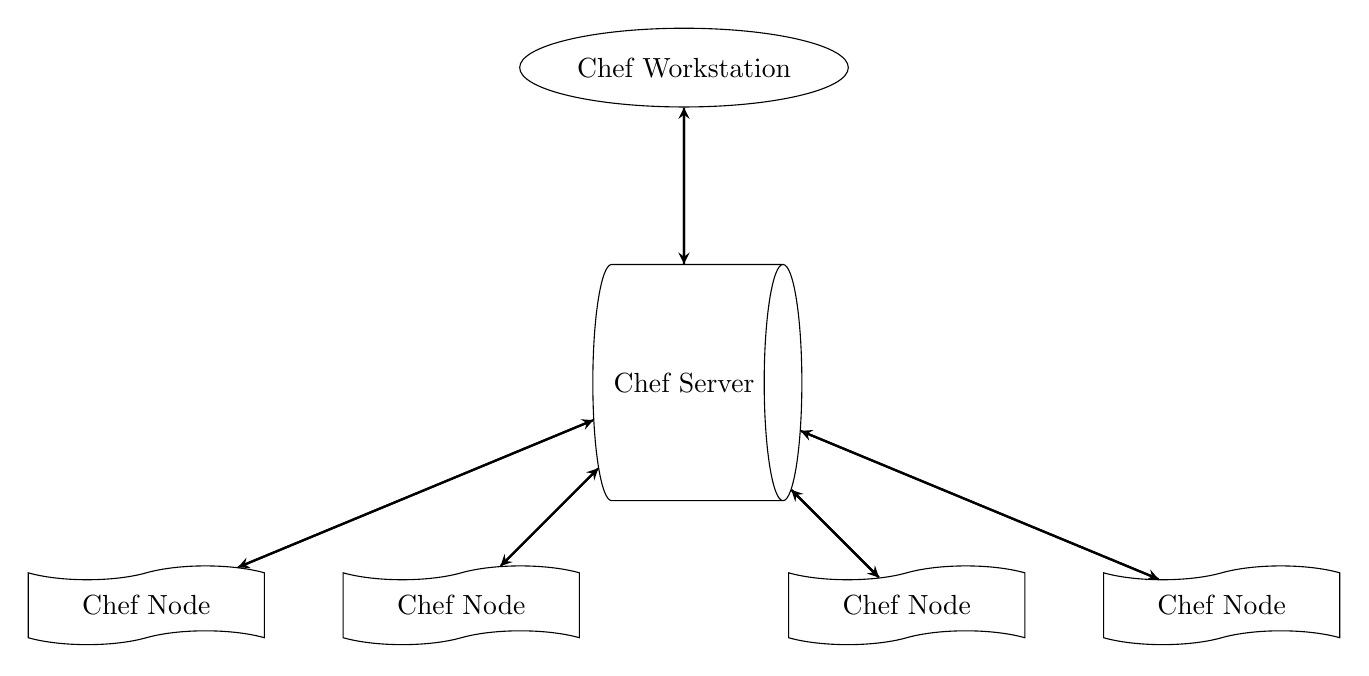
\begin{tikzpicture}[node distance=4cm]
\node (workstation) [workstation] {Chef Workstation};
\node (server) [server, below of=workstation] {Chef Server};
\node (cnode_one) [cnode, below left of=server] {Chef Node};
\node (cnode_two) [cnode, below right of=server] {Chef Node};
\node (cnode_three) [cnode, right of=cnode_two] {Chef Node};
\node (cnode_four) [cnode, left of=cnode_one] {Chef Node};

\draw [arrow] (workstation) -- node {} (server);
\draw [arrow] (server) -- node {} (workstation);

\draw [arrow] (cnode_one) -- node {} (server);
\draw [arrow] (server) -- node {} (cnode_one);
\draw [arrow] (cnode_two) -- node {} (server);
\draw [arrow] (server) -- node {} (cnode_two);
\draw [arrow] (cnode_three) -- node {} (server);
\draw [arrow] (server) -- node {} (cnode_three);
\draw [arrow] (cnode_four) -- node {} (server);
\draw [arrow] (server) -- node {} (cnode_four);

\end{tikzpicture}
\end{center}
\caption{Architecture of Chef} \label{fig:1}
\end{figure}

\newpage
\subsection{Features}
Chef provides the following features:
\begin{itemize}
\item
Automatic Backup
\item
Automatic Notifications
\item
Compliance Management
\item
Configuration Management
\item
Data Recovery
\item
Data Visualization
\item
Real Time Analytics
\item
Real Time Data
\item
Real Time Monitoring
\item
Real Time Notifications
\item
Real Time Reporting
\item
Real Time Updates
\item
Server Monitoring

\end{itemize}

\subsection{Official Website}
The official website for Chef is located at \href{https://www.chef.io}{https://www.chef.io}.
\subsection{Latest Version}
As of January 28, 2019, the latest stable release of the Chef client is v14.10.9.\\
As of October 15, 2018, the latest stable release of the Chef server is v12.18.14.
\subsection{Advantages}
Advantages of using Chef include:
\begin{enumerate}
\item
There is a low barrier for entry. Chef uses native Ruby language for configuration. This means that it can be easily picked up by anyone who has some development experience.
\item
It integrates execellently with cloud. Using the knife utility, Chef can be easily integrated with most existing cloud technologies. It is a suitable tools for organizations that wish to distribute their infrastructure on multi-cloud environment. 
\item
Chef can help organizations to accelerate software delivery, i.e. how quickly the software is able to be changed in response to new requirements or conditions. 
\item
Helps organizations to catch bugs and issues before they occur. Infrastructure automation increases a system's resiliency just as much as it accelerates delivery speed. 
\item
Improving risk management - the \textit{quality} of changes made to the software.
\item
When using Chef, you can deliver all your infrastructure everywhere continuously.
\end{enumerate}
\subsection{Disadvantages}
Some disadvantages include:
\begin{enumerate}
\item
Cookbooks require constant monitoring so that the people who are working do not cause any issues with them. 
\item
Only Chef solo is available. 
\item
Currently, Chef is only a good fit for Amazon Web Services Cloud. 
\item
Someone who is not familiar with Ruby may have a hard time learning it.
\item
There is currently a lack of proper documentation.
\end{enumerate}

\newpage
\section{Ansible}
Ansible is an open-source automation tool, or platform, used for IT tasks such as configuration management, application deployment, intraservice orchestration, and provisioning. Thus, simplifying complex tasks, making the jobs of developers more manageable and allowing them to focus attention on other tasks that addd value to their organization. 

\subsection{Components}
\begin{itemize}
\item
\textbf{Plays}\\
Playbooks contain plays. Plays are essentially groups of tasks that are performed on defined hosts to enforce your defined functions. Each play must specify a host or group of hosts. 
\item
\textbf{Tasks}\\
Tasks are actions carried out by playbooks. A task definition can contain modules such as yum, git, service, and copy.
\item
\textbf{Roles}\\
A role is the way Ansible bundles automation content to make it reusable. Roles are organizational components that can be assigned to a set of hosts to organize tasks. Therefore, instead of creating a monolithic playbook, we can create multiple roles, with each role assigned to complete a unit of work. For example: a webserver role can be defined to install Apache and Varnish on a specified group of servers.
\item
\textbf{Handlers}\\
Handlers are very similar to tasks. The major difference is that a handler will be executed only when it is called by an event. The handler is called by the [notify] directive. The name of the notify directive and the handler must be the same. 
\item
\textbf{Templates}\\
Templates files are based on Python's Jinja2 template engine and have a .j2 extension. If necessary, you can place contents of your index.html file into a template file. But the real power of templates is comes when variables are used. Ansible's [facts] can be used in template files, and users can even call custom variables.
\item
\textbf{Variables}\\
You can include custom-made variables in your playbooks. Variables can be defined in five (5) different ways:
\begin{enumerate}
\item
Variables defined under the vars\_file attribute.
\item
Variables defined in \textit{role}/vars/apache-install.yml
\item
Variables passed through the command line.
\item
Variables defined in the play under vars.
\item
Variables defined in group\_vars/ directory.
\end{enumerate}
\end{itemize}

\subsection{Architecture}
The architecture that makes up Ansible is as follows:
\begin{itemize}
\item
\textbf{Modules}\\
Ansible works by connecting to your nodes and pushing out small programs, called "Ansible Modules" to them. These programs are written to be resource of the desired state of the system. Ansible then executes these modules (over SSH by default), and removes them when finished. Your library of modules can reside on any machine, and there are no servers, daemons, or databases required. Typically you'll work with your favorite terminal program, a text editor, and probably a version control system to keep track of changes to your content.
\item
\textbf{Plugins}\\
Plugins are pieces of code that augment Ansible's core functionality.
\item
\textbf{Inventory}\\
The inventory is a configuration file where you define the host information.
\item
\textbf{Playbooks}\\
A playbook is where users define how to apply policies, declare configurations, orchestrate steps and launch tasks either synchronously or asynchronously on their servers.  Each playbook is composed of one or more plays. Playbooks are normally maintained and managed in a version control system like Git. They are expressed in YAML (Yet Another Markup Language). In most cases - especially in enterprise environments - using Ansible playbooks is recommended.
\end{itemize}


\subsection{Features}
\begin{itemize}
\item
\textbf{Configuration Management}\\
Ansible is designed to be very simple, reliable, and consistent for configuration management. Users who are familiar with the field of Information Technology can usually get up and running fairly quickly with Ansible. Ansible configurations are simple data descriptions of infrastructure and are both by readable by humans and parsable by machines. A password or an SSH key is all that is needed to start managing systems. For example, if a user wants to install an updated version of a specific type of software on all the machines in their enterprise, all they need to do is write out all the IP addresses of the nodes (also called remote hosts) and write an Ansible playbook to install it on all the nodes, then run the playbook from their control machine.
\item
\textbf{Application Deployment}\\
Ansible also allows users to quickly and easily deploy multitier applications. Users do not need to write custom code to automate their systems; they simply need to list the tasks required to be done in a playbook, and Ansible will figure out how to get their systems to the state they want them to be in. In other words, users need not configure the applications on every machine manually. When a playbook is run from the user's control machine, Ansible uses SSH to communicate with the remote hosts and run all the commands (tasks).
\item
\textbf{Orchestration}
Orchestration involves bringing different elements into an efficiently-running, whole operation. For example, with application deployment, users need to manage the front-end and backend services, databases, networks, storage, and so on. They also need to ensure that all tasks are handled in the proper order. Ansible uses automated workflows, provisioning, and more to simplify the process of orchestration. Once the infrastructure has been defined using Ansible playbooks, that same orchestration can be used wherever it is needed. This is due largely to the portability of Ansible playbooks.
\item
\textbf{Security and Compliance}\\
As with application deployment, sitewide security policies (such as firewall rules) can be implemented along with other automated processes. If the security details on the control machine are configured and the associated playbook is run, all the remote hosts will automatically be updated with those details. Therefore, users will not need to monitor each machine for security compliance continually manually. For extra security, an admin's user ID and password are not retrievable in plain text on Ansible.
\item
\textbf{Cloud Provisioning}\\
The first step in automating your applications' life cycle is automating the provisioning of your infrastructure. With Ansible, you can provision cloud platforms, virtualized hosts, network devices, and bare-metal servers.
\end{itemize}

\subsection{Official Website}
The official website for Ansible is \href{https://www.ansible.com/}{https://www.ansible.com/}.
\subsection{Latest Version}
As of June 14, 2018, the latest version of Ansible is 2.5.5.
\subsection{Advantages}
Ansible offers the following advantages:
\begin{enumerate}
\item
\textit{Free:} Ansible is an open-source tool.
\item
\textit{Very simple to set up and use:} No special coding skills are necessary to use playbooks in Ansible.
\item
\textit{Powerful:} Ansible lets you model highly complex IT workflows.
\item
\textit{Flexible:} The entire application environment can be orchestrated no matter where it is deployed. It can also be customized to suit user's needs.
\item
\textit{Agentless:} No other software or firewall ports need to be installed on the client systems users wish to automate. Setting up a separate management structure is also unnecessary. 
\item
\textit{Efficient:} Because there is no need to install any extra software, there is more room for application resources on the server.
\end{enumerate}
\subsection{Disadvantages}
Disadvantages of Ansible include:
\begin{enumerate}
\item
\textbf{No Notion of State:} Unlike comparable automation tools, Ansible has no notion of state. Since it does not keep track of dependencies, the tool simply executes a sequential series of tasks, stopping when it finishes, fails or encounters an error. Many users tend to prefer that their automation tool maintain an extensive catalog for ordering, allowing them to reach a defined state regardless of any variance in environmental conditions.
\item
\textbf{Nascent Windows Support}: Ansible suports both Unix/Linux and Windows nodes. For Windows nodes it uses native powershell remoting (as opposed to SSH), and a Linux control machine is still required for managing Windows hosts. Ansible is still early in its efforts to extend support for Windows. 
\item
\textbf{Minimal Enterprise Support Experience:} Ansible has had considerably less experience working with large enterprises than competitors like Chef and Puppet. 
\item
\textbf{Relatively New:} Ansible has not been around as long as competitors such as Chef or Puppet. As a result, it has the smallest developer/user community and has the least easily accessible material on the internet for self-help and troubleshooting. Less time on the market means more bugs, edge scenarios, and software issues have perhaps not yet appeared. 
\end{enumerate}


\newpage
\section{Fuel}
\subsection{Components}
\subsection{Architecture}
\subsection{Features}
\subsection{Official Website}
\subsection{Latest Version}
\subsection{Advantages}
\subsection{Disadvantages}

\newpage
\section{Puppet}
\subsection{Components}
\subsection{Architecture}
\subsection{Features}
\subsection{Official Website}
\subsection{Latest Version}
\subsection{Advantages}
\subsection{Disadvantages}

\newpage
\section{Compass}
\subsection{Components}
\subsection{Architecture}
\subsection{Features}
\subsection{Official Website}
\subsection{Latest Version}
\subsection{Advantages}
\subsection{Disadvantages}

\newpage
\section{References NEED TO FORMAT PROPERLY}
\href{https://shadow-soft.com/chef-benefits/}{https://shadow-soft.com/chef-benefits/}\\
\href{https://www.tutorialspoint.com/chef/chef_overview.htm}{https://www.tutorialspoint.com/chef/chef\_overview.htm}\\
\href{https://www.linode.com/docs/applications/configuration-management/beginners-guide-chef/}{https://www.linode.com/docs/applications/configuration-management/beginners-guide-chef/}\\
\href{https://www.simplilearn.com/what-is-ansible-article}{https://www.simplilearn.com/what-is-ansible-article}\\
\href{https://cloudacademy.com/blog/ansible-aws/}{https://cloudacademy.com/blog/ansible-aws/}


\end{document}